%%==================================================
%% chapter01.tex for BIT Master Thesis
%% modified by yang yating
%% version: 0.1
%% last update: Dec 25th, 2016
%%==================================================
\chapter{绪论}
\label{chap:intro}
\section{研究背景与研究意义}

随着数字化技术的高速发展,以互联网为主要传播载体的各种信息资源呈现出过载化和爆炸化发展趋势。在这些形式多样的信息资源中,以新闻报道、电子刊物和社交内容等为代表的海量文本信息占据了不可或缺的地位,然而其主要以非结构方式存在,信息密度相对不高,不利于知识的进一步存储、转化与应用。为了提升对于文本信息的利用效率,大量的信息抽取(Information Extraction)\cite{peng2023fsuie,jia2023modeling,黄河燕2023融合实体和上下文信息的篇章关系抽取研究,蔡宇翔2024基于跨度边界感知的嵌套命名实体识别}研究工作聚焦于自动化和智能化地获取非结构文本内容中的结构化知识数据。

近年来,事件抽取(Event Extraction)成为了信息抽取领域新的研究热点。事件抽取旨在从非结构的纯文本中抽取状态发生改变的事物,可表示为在特定时间、特定地点发生涉及若干参与者(物体)动作的结构化语义信息,其广泛应用于语言理解的不同领域,如事实核查~\cite{wu2022cross,liu2023covid}、信息检索~\cite{kuhnle2021reinforcement,zhang2021drl4ir}、智能问答~\cite{boyd2020question,wen2021resin}、推荐系统~\cite{liu2017cpmf,abdollahi2023laser}等。此外,利用事件抽取技术以及事件指代消解~\cite{lu2021span,lu2022end}、事件关系抽取~\cite{liu2020extracting,zhuang2023syntax}等后续任务构建的事件知识图谱区别于以实体为中心的传统静态知识描述~\cite{guan2023event},反映了逻辑社会的动态事件性知识,可以进一步增益相应的下游应用~\cite{cheng2020knowledge,souza2020event}。而且,以ChatGPT为代表的大语言模型虽然在多种自然语言处理任务中表现出类人的性能,但仍然受限于幻觉和缺乏显式知识建模~\cite{wu2023brief}。事件知识图谱作为幻觉检测和知识注入技术应用发展的重要基础之一~\cite{pan2023large},为探索解决大语言模型的此类局限提供了坚实支撑。

% 事件抽取检测一段文本中的事件及相关信息,一般包括事件的存在性、预定义类型信息、参与者和参与者与事件存在的预定义关系等。具体来说,在事件抽取中,研究工作普遍采用事件抽取以ACE~\footnote{https://www.ldc.upenn.edu/collaborations/past-projects/ace}为代表的评测项目中定义的事件术语,主要包括表达事情发生的事件触发词和表示参与者与属性的事件要素。

现有研究工作通常将事件抽取形式化处理为两阶段任务:事件检测和事件要素抽取。其中,事件检测任务识别出文本中触发事件的单词或者短语,并将其归类到正确的预定义事件类型上。而事件要素抽取任务旨在抽取出参与事件的实体提及以及对应的预定义事件要素类型。图\ref{example_chap1}展示了一个具体的事件抽取实例,事件检测任务首先识别出文本中的短语“辞去”触发了“辞职”事件,而事件要素抽取任务基于事件检测的结果进一步抽取出参与事件的实体提及“埃隆·马斯克”、“推特”和“首席执行官”以及对应的要素类型“人物”、“公司”和“职位”。

\begin{figure}[htp]
    \centering
   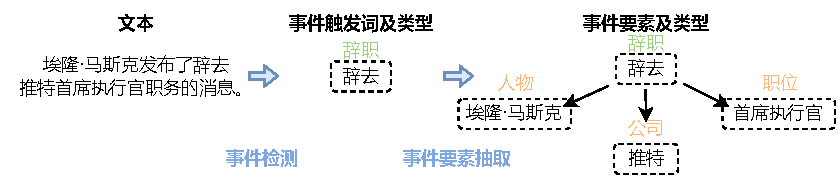
\includegraphics[width=1\linewidth]{figures/chap1/example_chap1.pdf}
   \caption{事件抽取实例}
   \label{example_chap1}
\end{figure}

随着深度学习技术的发展,这两阶段任务均取得相当优异的性能提升。然而,不管是针对事件检测还是事件要素抽取的研究,主要聚焦在特定的模型架构上进行,如循环神经网络、卷积神经网络、图神经网络和预训练语言模型等,忽略了任务中不同模型架构均普遍存在的数据依赖:(1)事件检测数据集中不存在事件的实例比例过高,这种数据不平衡依赖影响了不同模型架构识别事件的能力,从而进一步导致事件检测分类的错误;(2)事件要素抽取数据集中实体提及的类型与要素类型呈现出的强关联依赖,阻碍了不同模型架构更好地建模理解文本中的语义信息。此外,近年来随着各类文本信息资源呈现复杂化的演变趋势,越来越多的事件要素以跨越多个句子的方式出现,其对事件抽取中的事件要素抽取建模方式提出了新要求。因此,研究同时适用于句子级别和文档级别的事件要素抽取方法成为新的研究热点和挑战。然而,(3)现有研究无法在避免共有内在局限性的前提下,实现对不同级别文本中均存在的跨事件依赖关系进行有效构建与利用。

因此,研究事件抽取中的共性数据依赖,可以进一步增强基于不同类型神经网络架构和不同级别文本的现有事件抽取方法的性能表现,提升其作为结构化语义信息应用到不同语言智能化理解领域的质量,支撑事件知识图谱的构建。此外,本研究面向共性数据依赖的特点,赋予其适应新的事件抽取模型架构和建模范式的潜力,具备良好的扩展性。更为重要的是,本研究提出的共性数据依赖是各自所在子领域广泛存在但尚未引起重视的新挑战,具有广阔的深入研究前景。

\section{研究内容与主要贡献}

面对事件抽取系统中不同阶段存在的共性数据依赖,本文从不同的模型架构和文本范围出发,研究通用性的应对方法。其中,针对事件检测阶段普遍存在的数据不平衡依赖问题,提出了基于分类器自适应知识蒸馏的方法;针对事件要素抽取阶段普遍存在的实体类型过度依赖问题,提出了基于多角度对比学习的方法;针对将事件要素抽取扩展到多级别文本时普遍缺乏有效利用跨事件依赖关系的问题,提出了基于分离-融合范式的方法。如图\ref{subtask_relation}所示,上述研究内容覆盖了当前事件抽取系统的关键阶段和应用范围。接下来,具体阐述本文的研究内容和主要贡献如下:

\begin{figure}[htp]
    \centering
   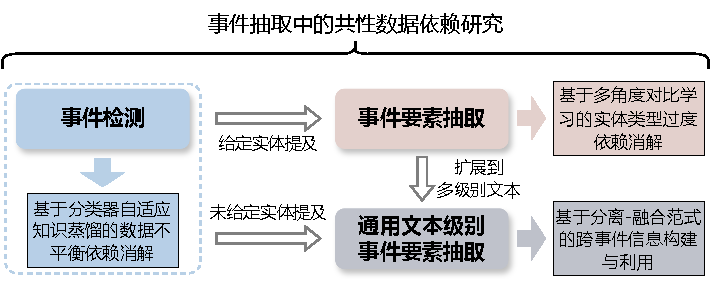
\includegraphics[width=0.8\linewidth]{figures/chap1/subtask-relation.pdf}
   \caption{研究内容关联图}
   \label{subtask_relation}
\end{figure}

\textbf{(1)基于分类器自适应知识蒸馏的数据不平衡依赖消解}

\textbf{问题阐述:}当前事件检测数据集存在严重的数据不平衡,限制了已有不同事件检测模型系统识别事件的能力,进一步降低了模型整体检测性能。针对该问题,相关研究特定于具体的模型架构和任务设计,依赖超参数以适应动态变化的数据不平衡程度,阻碍了可扩展性。

\textbf{研究内容:}针对上述问题,本文工作首先定义和引入句子级别识别信息,并验证该信息在消解数据不平衡依赖导致的性能下降方面的优势。基于此,研究利用知识蒸馏原理自动捕捉句子级别识别信息,提出在事件识别增强网络输入中增加对于句子级别识别信息的构建,并通过分类器参数引导事件检测网络从原始文本中自动学习该信息,实现事件检测性能的增强。

\textbf{主要贡献:}该研究为消解事件检测中存在的数据不平衡依赖问题提供了新颖的角度。与现有的消解方法基于具体数据不平衡程度\textbf{被动}地增强正样本或减弱负样本的训练权重不同,本文工作从数据不平衡依赖影响事件检测性能的方式出发,以此引入了句子级别识别信息进行\textbf{主动}地消解数据不平衡依赖导致的性能损失,并针对性地设计了知识蒸馏框架自动学习该信息。因此,这种主动方式实现了不依赖超参数而自主适应不同模型架构和数据不平衡程度的多维度通用数据不平衡依赖消解。

\textbf{(2)基于多角度对比学习的实体类型过度依赖消解}

\textbf{问题阐述:}不同的事件要素抽取模型在建模事件触发词与实体提及的复杂交互时,受益于实体提及类型信息,忽略了其与要素类型间的强关联性。该强关联性使得不同的事件要素抽取模型在建模中对于实体类型过度依赖,影响了事件要素类型的正确预测。

\textbf{研究内容:}针对上述问题,本文工作首先定义实体类型过度依赖问题并通过实验研究该问题在不同事件要素抽取架构中的存在性。基于此,研究利用监督对比学习分别从正样本和负样本两个角度进行实体类型过度依赖消解,并构建循环训练策略,以实现不同角度消解的高效协作。

\textbf{主要贡献:}该研究提供了在事件要素抽取中利用实体类型信息的新思路。与现有方法关注实体类型信息的\textbf{正面增益}不同,本文工作从实体类型与要素类型的数据特点出发,清晰地定义了实体类型过度依赖,并验证了其在不同模型架构中存在的普遍性,评估了其对于要素类型预测性能产生的\textbf{负面影响}。为了消解该问题,本文工作提出了两种新的监督对比学习方法,聚焦从不同角度减少实例特征表示对于实体类型的依赖性,提升整体文本语义信息的建模质量,通用有效地消解了实体类型过度依赖导致的性能损失。

\textbf{(3)基于分离-融合范式的跨事件信息构建与利用}

\textbf{问题阐述:}当前适用于不同文本级别的事件要素抽取方法存在各自的局限性,而基于多词元链接的建模方法能够有效避免这些局限性并表现出良好的性能潜力。然而,在现有的多词元链接方法中,单一事件建模方式缺乏利用跨事件依赖关系,多事件建模方式需要增加编码序列和链接操作,导致了更多预测错误的积累。

\textbf{研究内容:}针对上述问题,研究结合不同多词元链接建模方式的各自优势,提出分离-融合抽取范式,将跨事件信息获取和事件要素抽取的建模过程进行分离,再将获取的跨事件信息融合到目标事件的要素预测中。遵循该研究范式,进一步提出相应的多词元链接模型,通过设计不同的多词元链接构建和两阶段融合机制,以实现建模不同事件间关联依赖性的同时,保持了高效直接的要素链接推理。

\textbf{主要贡献:}该研究为利用多词元链接进行通用文本级别事件要素抽取构建了新范式。与现有事件建模方式存在\textbf{各自优势}不同,本文工作提出的分离-融合抽取范式,构建了跨事件信息获取和事件要素抽取过程的分离再融合,从而实现了现有不同事件建模方式优势的\textbf{高效统一}。在该范式的指导下,提出了新的多词元链接模型,有效地构建与利用了不同文本级别事件要素抽取共有的跨事件依赖信息。

\section{论文组织结构}

本文工作面向事件抽取系统存在的共性数据依赖,根据\textbf{规划研究目标$\Rightarrow$明确研究内容$\Rightarrow$介绍现有工作$\Rightarrow$分析共性问题$\Rightarrow$阐述技术路线$\Rightarrow$总结研究成果}的行文结构,阐明相应的研究解决方法。如图\ref{organization}所示,将全文划分为六个章节,具体组织安排如下:

\begin{figure}[]
    \centering
   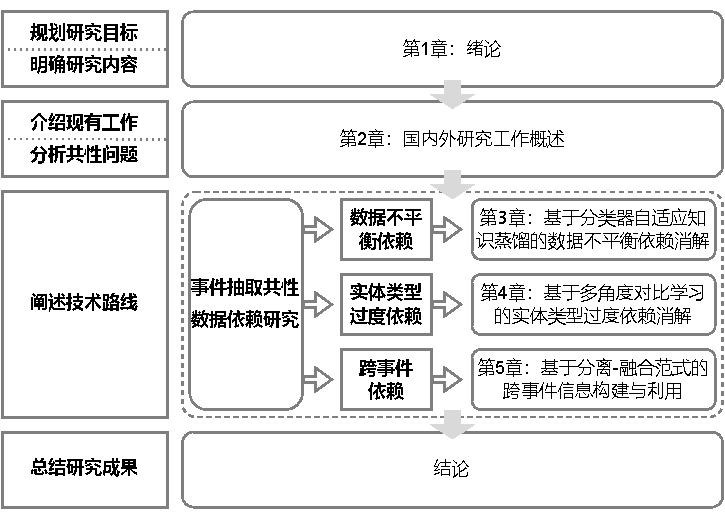
\includegraphics[width=1\linewidth]{figures/chap1/organization.pdf}
   \caption{论文组织结构示意图}
   \label{organization}
\end{figure}

第一章为绪论,介绍了事件抽取任务的研究背景和意义,概述存在于该任务中的共性数据依赖,提炼相应的研究内容和贡献。

第二章为国内外研究工作概述,按照事件抽取系统中的不同阶段分别梳理发展脉络,分析存在的研究问题,归纳研究思路。

第三章围绕事件检测中的数据不平衡依赖消解,研究数据不平衡问题影响整体性能的原因与方式,验证句子级别识别信息在消解其性能损失方面的有效性,进而基于分类器自适应引导的知识蒸馏方法,自动从原始文本中捕捉句子级别信息,实现模型架构通用的数据不平衡自动消解框架。

第四章围绕事件要素抽取中的实体类型过度依赖消解,研究从不同角度消解事件要素抽取建模时对于实体类型信息的过度依赖,通过监督对比学习技术分别从正样本和负样本角度减少实体类型对于实例特征表示的过度影响,并利用循环训练策略优化消解过程,实现文本语义信息建模质量的提升。

第五章围绕通用文本级别事件要素抽取中的跨事件信息构建与利用,研究融合不同多词元链接模型建模事件要素的优势,构建两种多词元链接和两阶段融合机制,以实现跨事件信息获取和事件要素抽取过程的分离再融合,在有效构建事件依赖的同时,保持单事件建模的简单链接预测,提升通用事件要素抽取系统的性能。

最后一章为结论,总结本文研究工作成果,并展望进一步的研究计划。

